\section{Literature Review}

\subsection{Automated Redistricting Algorithms}

- Explain purpose of these

- Give some of the first examples

- My research uses three of these, go in depth explaining them. 

\subsubsection{Markov Chain Monte Carlo}

The first automated redistricting algorithm that I'm going to discuss in detail is an implementation of a statistical method known as "Markov Chain Monte Carlo," henceforth MCMC \parencite{fifield2020}.\footnote{I will refer to the \emph{redistricting algorithm} that uses Markov Chain Monte Carlo as "MCMC," rather than the \emph{statistical method} Markov Monte Carlo.} The following overview is meant to provide a high-level understand of how the basic algorithm works. Since the purpose of my research is to compare the \emph{outputs}, that is the redistricting plans, generated by these algorithms, \emph{rather than the algorithms themselves}, a rigorous understanding of the algorithms is not a prerequisite.\footnote{Please see the section "The Proposed Methodology" in the paper for an in-depth, mathematically-rigorous explanation. \parencite[2]{fifield2020}}.

\begin{figure}
    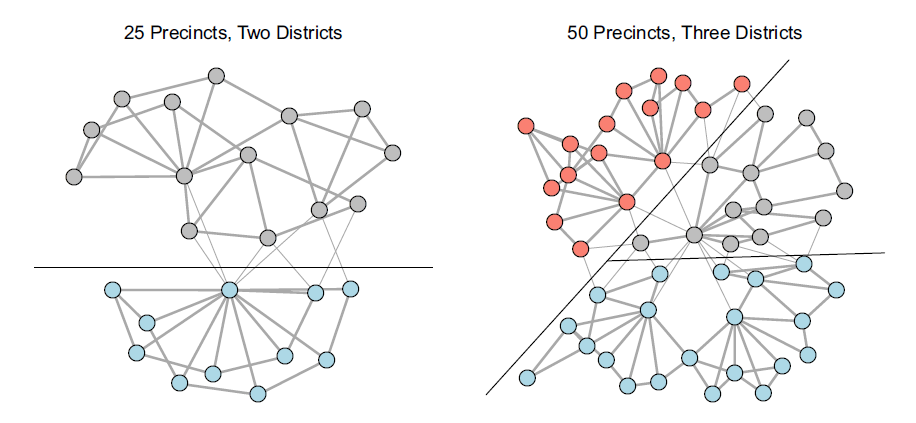
\includegraphics[width=\linewidth]{img/graphcut.png}
    \caption{Representation of redistricting as graph cutting. Every node is a precinct, and nodes that share an edge are known to be adjacent precincts. MCMC "cuts away" edges between nodes until islands of districts are formed. \parencite[3]{fifield2020}}
    \label{fig:graphcut}
\end{figure}

MCMC conceptualizes the problem of redistricting precincts as a graph-cutting problem. For the uninitiated, a graph is a network of different interconnected points, where the points are called "nodes" and the lines connecting them are called "edges" \parencite{fifield2020}. MCMC represents every precinct as a node, and it draws an edge between nodes where the corresponding precincts are adjacent. Since the goal of redistricting is to assign every precinct a district, MCMC imagines that edges between nodes are "cut" until "islands" (known as "sub graphs") are formed, which each is disconnected from the rest. The disconnected "sub graphs" then become the districts. Figure \ref{fig:graphcut} provides a nice visualization of this representation with a sample set of 50 precincts. \parencite{fifield2020}

\begin{figure}
    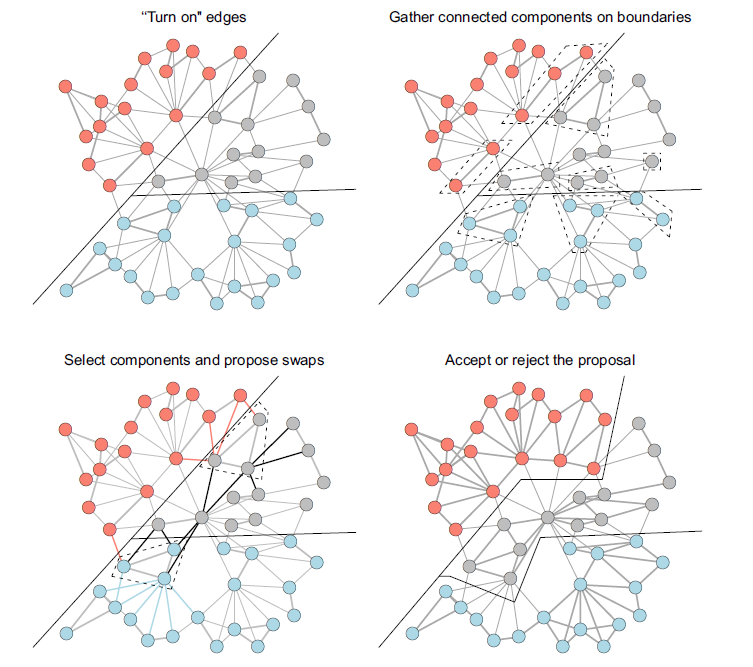
\includegraphics[width=0.75\linewidth]{img/swaps.png}
    \caption{Representation of MCMC algorithm. \parencite[4]{fifield2020}}
    \label{fig:swaps}
\end{figure}

Now that the representation used by MCMC has been established, we can discuss the specifics of the algorithm. Figure \ref{fig:swaps} visualizes the steps in this algorithm. The basic MCMC algorithm begins with a valid redistricting plan, such as the one currently in use, and randomly decides to "turn on" some edges in the graph. Then, the nodes (precincts) that are connected by these "turned on" edges and are located on the boundary of a district are identified. Then, these highlighted graph components are "nominated" for a swap across the district boundary based on some probability, provided that this swap would not break the district into two. Lastly, this new proposed redistricting plan is either accepted or rejected based on some "acceptance probability." This process is repeated as many times as desired. \parencite{fifield2020}.

MCMC in its current form allows for further constraint of this algorithm, particularly with regard to the relative population size and compactness of each district. \parencite[6]{fifield2020} The explanation of this algorithm is beyond the scope of this paper. 

\subsubsection{Sequential Monte Carlo}

The second automated redistricting algorithm that I'm going to discuss is an implementation of a statistical method known as "Sequential Monte Carlo," henceforth SMC \parencite{mccartan2020}.\footnote{I will refer to the \emph{redistricting algorithm} that uses Sequential Monte Carlo as "SMCMC," rather than the \emph{statistical method} Sequential Monte Carlo.} The following overview is meant to provide a high-level understand of how the basic algorithm works. \footnote{Please see the section "The Proposed Algorithm" in the paper for an in-depth, mathematically-rigorous explanation. \parencite[13]{mccartan2020}}.

\begin{figure}
    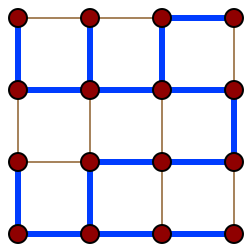
\includegraphics[width=0.3\linewidth]{img/4x4_grid_spanning_tree.png}
    \caption{An example spanning tree. The spanning tree consists of all nodes and the blue edges, where the complete graph includes the grid edges as well. \parencite{eppstein2007}}
    \label{fig:spantree}
\end{figure}

Just like MCMC, SMC conceptualizes the electoral map as a mathematical graph with precincts as nodes and edges connecting geographically-adjacent precincts. It also uses this graph-cutting concept, but SMC specifically uses something called a "spanning tree" (see Figure \ref{fig:spantree}), which is a graph that is connected by the minimum number of possible edges\footnote{Put another way, if any edge is cut from the graph, the graph will be split into two sub graphs.}. 

\begin{figure}
    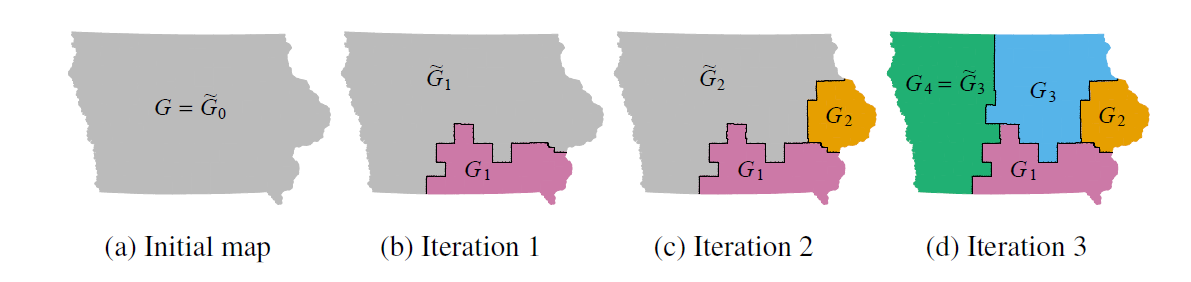
\includegraphics[width=\linewidth]{img/smc.PNG}
    \caption{Representation of splitting procedure of SMC. Every node is a precinct, and nodes that share an edge are known to be adjacent precincts. MCMC "cuts away" edges between nodes until islands of districts are formed. \parencite[14]{mccartan2020}}
    \label{fig:smc}
\end{figure}

Figure \ref{fig:smc} visualizes the iterative splitting procedure used by SMC. First, compute the deviation from the target precinct population for each subgraph generated by cutting each edge in the spanning tree. Then, randomly cut one of the edges, creating two new subgraphs\footnote{Technically they're spanning trees, which are known as a spanning forest in the plural.} If the smaller subgraph meets the population and compactness requirements, then it's accepted as the first district, and the splitting procedure is repeated with the other subgraph. 

This process generates the possible redistricting plans that satisfy the requirements. For more details, please refer to \textcite{mccartan2020}.

\subsubsection{Compact Random Seed Growth}

The final automated redistricting algorithm that I'm comparing is called Compact Random Seed Growth, henceforth referred to as "CRSG" and was proposed by \textcite{chen2013}. Its objective is to generate a set of districts that fall within a certain population constraint and are reasonably compact using only the geography and total population of each precinct \parencite{chen2013}. The following is a high-level explanation of the algorithm.\footnote{For more details, please refer to \textcite[249-50]{chen2013}.} 

CRSG begins with declaring that every precinct is it's own district. A random precinct is then chosen, and then its geographically-closest\footnote{The geographically-closest precinct is the neighboring precinct with the smallest distance from its centroid to the seed precinct's centroid} neighbor is merged with it, creating one fewer district. This process is repeated until you arrive at the desired number of districts. \parencite[249-50]{chen2013}

After this procedure, the districts are somewhat compact due to the geographic proximity requirement, but there is no guarantee that the districts are within the required population percentage of each other. 

To satisfy the population parity requirements, CRSG does the following. First, it identifies the two adjacent districts that have the greatest difference in total population. Then the precinct in the more-populous district that is furthest from the center of said district is reassigned to the less-populous district.\footnote{Provided that this reassignment doesn't break either district into parts.} This process is repeated until all of the districts are within some desired percentage of the mean district population.\textcite[249-50]{chen2013}.

One run of CRSG will produce one set of districts, but separate runs of CRSG with the same input data may produce slightly different districts given the random choice of districts to merge in the first pass of the algorithm. 

\subsection{Measures of Partisan Fairness}

\textcite{katz2020} brings mathematical rigor to the various proposed metrics for measuring partisan symmetry. 

\subsubsection{Partisan Symmetry}

A legislative is said to have partisan symmetry if both parties can receive $m$ proportion of the overall votes and therefore have $n$ proportion of the seats in the legislative body.An example would be that if Republicans win 60\% of the votes but control 65\% of the seats, then in a symmetrical system, Democrats should also be able to control 65\% of the seats by winning 60\% of the votes. \textcite{katz2020}

Partisan Bias is any deviation from partisan symmetry. If partisan bias is greater than 0, it is biased towards Democrats, and it's biased towards Republicans if less than 0. \parencite{katz2020}

\begin{figure}
    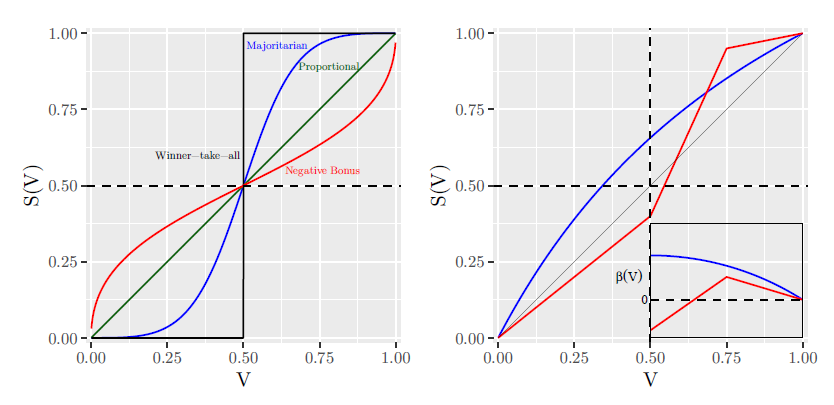
\includegraphics[width=0.8\linewidth]{img/seatsvotes.png}
    \caption{Types of Seats-Votes Curves. Left panel: Symmetric (fair) curves with differing
    levels of electoral responsiveness. Right panel: Asymmetric (biased) curves, including
    one consistently biased toward the Democrats (blue) and one with biases favoring different
    parties depending on V (red); the inset graph is for (V ) for V 2 [0:5; 1] with the vertical
    axis scaled to be the same as the main plot, and lines color coded to the seats-votes curves. \parencite[175]{katz2020}}
    \label{fig:seatsvotes1}
\end{figure}

Partisan symmetry is usually observed by plotting a "seats-votes curve." This plot has $V$, the proportion of the overall votes won by the party, on the x-axis, and $S(V)$, the proportion of the seats won by the party, on the y-axis. Figure \ref{fig:seatsvotes1} \parencite[175]{katz2020} illustrates several hypothetical seats-votes curves.

Naturally, it's very rare to observe the necessary electoral outcomes under the same electoral system in order to determine partisan symmetry. (i.e., it's very rare for two parties to tie one year, have one win 51\% of the total votes the next year, and then win 49\% of the votes the following year.)

In practice, one can estimate a seats-votes curve using the principle of uniform partisan swing.

\paragraph{Uniform Partisan Swing}

Uniform partisan swing is the principle that when the overall vote between different elections under the same electoral system, the vote share at the district level also usually changes by the same $dV$. \textcite{katz2020} Empirically verified this to be true in 646 different elections. 

Thus, given a list of vote proportions per district ${v_1, v_2, v_3, ...}$ from one election, one can adjust each vote proportion by an arbitrarily small $dV$ until the seats share $S(V)$ is covered from 0 to 1. \parencite{katz2020}.

An example of such a curve is shown in Figure \ref{fig:seatsvotesups1}

\begin{figure}
    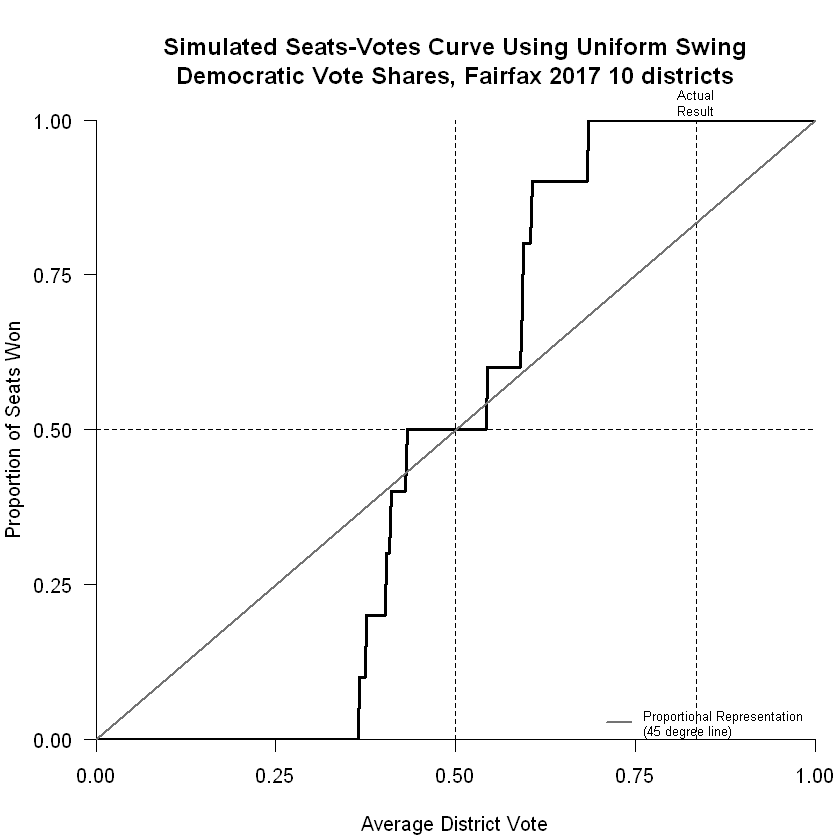
\includegraphics[width=0.5\linewidth]{img/seatsvotesups.png}
    \caption{Sample seats-votes curve generated using uniform partisan swing. Ignore title. \parencite[175]{katz2020}}
    \label{fig:seatsvotesups1}
\end{figure}

\subsubsection{Mean-Median Difference}

The mean-median difference $MM$ is defined as the difference between the mean Democratic vote share (DVS) of each district and median democratic vote share of each district (first proposed by \textcite{mcdonald2015}). If $MM = 0$, the districts are said to be fair. 

\textcite{katz2020} finds that the mean-median difference is a reliable estimator of partisan bias when the average DVS is 0.5. In the language of seats-votes curves, this means it can detect partisan bias at the average DVS = 0.5 level, but not at any other. Essentially, they find that mean-median difference is a reliable estimate of partisan bias as the average DVS changes, but not as the seat share changes (i.e. can measure bias along x-axis but not y-axis of seats-votes curve). \parencite[27-9]{katz2020}

\subsection{Measures of Compactness}

A universal requirement of districts is that they be "reasonably compact." There is no legally accepted universal definition of compactness, and the scholarship is not united behind one measure either. The following is a brief overview of several different, commonly-used compactness measures that vary in approach, benefits, and weaknesses. 

\subsubsection{Polsby-Popper Score}

Our first measure of district compactness is the Polsby-Popper score. \textcite{polsby1991} introduces this measure of compactness first development in paleontology to the problem of gerrymandering. It calculates the ratio of the area of the district to the area of the circle with the same perimeter as the district. It is calculated as follows.

\begin{equation}
    PP(d) = \frac{4 \pi A(d)}{P(d)^2}
\end{equation}

where $d$ is the district, $A(d)$ is the area of the districts, $P(d)$ is the perimeter of the districts, and $PP(d)$ is the Polsby-Popper score \parencite{cox1927,polsby1991}. The score will range from 0 to 1, where 0 is a lack of compactness and 1 is the most-compact district \parencite{polsby1991}.

Limitations and criticisms of this measure include that it is very sensitive to both geography and map resolution. Particularly near coastlines, even the most compact districts can have Polsby-Popper scores that are lower than gerrymandered districts which don't border coastlines. At finer resolutions, the same district will have a lower Polsby-Popper score as the perimeter increases. \parencite[12]{mccartan2020}.

\subsubsection{Schwartzberg Score}

The Schwartzberg score is very similar to the Polsby-Popper Score, but it calculates the ratio of of the perimeter of the district to the perimeter of a circle with the same area as the district \parencite{schwartzberg1966}. It is calculated as follows. 

\begin{equation}
    S(d) = \frac{P(d)}{2 \pi \sqrt{\frac{A(d)}{\pi}}}
\end{equation}

where $S(d)$ is the Schwartzberg score. $S(d)$ ranges from 0 to 1, with 0 again being the least compact and 1 being the most compact district. 

While the Schwartzberg measure is very sensitive to almost all forms of noncompactness (eg. spikes, cross-shapes, etc.) \parencite[301]{polsby1991}, it is hampered by the same issues as the Polsby-Popper score, namely that it incorrectly characterizes coastal districts as gerrymandered and is sensitive to resolution. 

\subsubsection{Length-Width Score}

The Length-Width score requires a minimum-bounding rectangle to be drawn around the district. The length-width score is the ratio of the shorter side of the rectangle to the longer side (i.e. a district encapsulated by a square would have a score of 1) \parencite{harris1964}. Just like the previous two measures, the Length-Width score ranges from 0 to 1, with a score of 1 indicating the most compact district. 

Criticisms of this measure include that it is not sensitive to perimeter changes, meaning that a square district and a square district of the same size with many indentations would have the same compactness score \parencite{polsby1991}.

\subsubsection{Convex Hull Score}

The Convex Hull score calculates the ratio between the area of the district and the area of the convex hull of the district. A convex hull is the smallest possible polygon with entirely acute interior angles that contains the desired points. It again ranges from 0 to 1, with 1 being the most compact district. \parencite{maceachren1985}

Criticism of the Convex Hull score primarily address that coastal districts may have lower scores even though they may be as compact as possible given their geographic constraints.

\subsubsection{Reock Score}

The Reock Score is the ratio between the area of the district and the area of the smallest possible circle that encloses it, known as the minimum bounding circle. It is very similar to the Length-Width score and the Convex-Hull score, and it also ranges from 0 to 1, with 1 indicating the most compact district, a circle. \parencite{reock1961}

Criticism of the Reock Score include that it does not account for internal indentations associated with "salamander-like" districts, just like the Length-Width score \parencite{maceachren1985}. 

\subsubsection{Boyce-Clark Index}

The Boyce-Clark Index scores the compactness of districts using the length of the radii from the geometric centroid, or "center of mass", of the district. It is computed as 

\begin{equation}
    1 - \sum_{1}^{16}\{\frac{|\frac{r_i}{\sum_ir_i}*100-6.25 |\}}{200}
\end{equation},

where $r_i$ are the 16 individual radii. A perfect circle will have a Boyce-Clark index of 1. \parencite{boyce1964,fifield2020d}

Criticisms of this measure include that it would score districts that must naturally be concave, possibly due to coastal geography, lower than is fair. Since the resolution is 16 radii, it is also sensitive to the orientation of the district \parencite{boyce1964}.

\subsubsection{Fryer-Holden Score}

The Fryer-Holden score takes a different approach to quantifying compactness, as it takes the population of each precinct into account. This score is "based on the distance between voters within the same political district in a state relative to the minimum such distance achievable by any districting plan in that state" \parencite[2]{fryer2007}. A score of 1 indicates a compact district. 

This measure is robust to some of the weaknesses of the previous measures, namely that it isn't affected by coastal geography, map resolution, or population density. It can also be compared across states. \parencite{fryer2007}

\subsubsection{Edge-Cut Compactness}

Edge-Cut Compactness takes a graph-theory perspective to district compactness. Imagine a graph where each precinct is a node, some vertex of the graph, and every adjacent precinct shares an edge, a line connecting the points. The Edge-Cut compactness score is the number of edges that must be "cut" (removed) from the original graph to form subgraphs, or districts. The theory is that compacter districts will require fewer edges to be cut. \parencite{dube2016} If normalized to the number of edges and subtracted from 1, a score of 1 indicates the most compact district. 

Benefits of this measure include that it is unaffected by political or natural geography and map resolution, as well as population density \parencite[11]{mccartan2020}. 